\documentclass[10pt,a4paper]{article}
\usepackage[margin=16mm]{geometry}
\usepackage[T1]{fontenc}
\usepackage[utf8]{inputenc}
\usepackage{amsmath,amssymb,tikz,adjustbox,longtable,booktabs}
\usepackage[colorlinks=true,linkcolor=blue]{hyperref}
\tikzset{ewstrand/.style={line width=.85pt,line cap=round,line join=round},ewletter/.style={font=\scriptsize,inner sep=1pt}}
\setlength{\parindent}{0pt}
\setlength{\parskip}{5pt}
\definecolor{ewcolor0}{HTML}{C43136}
\definecolor{ewcolor1}{HTML}{2268B0}
\definecolor{ewcolor2}{HTML}{16804A}
\begin{document}
{\Large\bfseries Elias--Williamson morphism}\par
A coefficient multiplies on the left. 
The requested morphism is \(F=N_{0}\). Shared expressions are named below.\par
\clearpage
{\large\bfseries Node 0}\par
\(N_{0}:B_{\text{t}\,\text{s}\,\text{t}\,\text{u}\,\text{u}}\to B_{\text{s}\,\text{u}\,\text{u}\,\text{s}\,\text{s}}\).\par
\begin{center}\begin{adjustbox}{max width=.96\linewidth,max height=19cm}
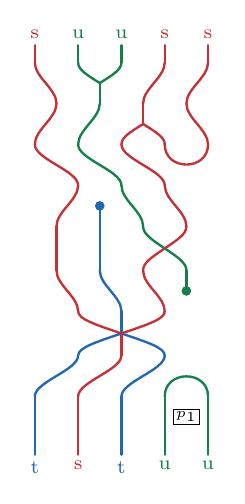
\begin{tikzpicture}[baseline=(current bounding box.center)]
\node[ewletter,text=ewcolor1,anchor=north] at (-1.1000,-0.0400) {$\text{t}$};
\node[ewletter,text=ewcolor0,anchor=north] at (-0.5500,-0.0400) {$\text{s}$};
\node[ewletter,text=ewcolor1,anchor=north] at (0.0000,-0.0400) {$\text{t}$};
\node[ewletter,text=ewcolor2,anchor=north] at (0.5500,-0.0400) {$\text{u}$};
\node[ewletter,text=ewcolor2,anchor=north] at (1.1000,-0.0400) {$\text{u}$};
\draw[ewstrand,ewcolor1] (-1.1000,0.0000) .. controls (-1.1000,0.0792) and (-1.1000,0.1408) .. (-1.1000,0.2200);
\draw[ewstrand,ewcolor0] (-0.5500,0.0000) .. controls (-0.5500,0.0792) and (-0.5500,0.1408) .. (-0.5500,0.2200);
\draw[ewstrand,ewcolor1] (0.0000,0.0000) .. controls (0.0000,0.0792) and (0.0000,0.1408) .. (0.0000,0.2200);
\draw[ewstrand,ewcolor2] (0.5500,0.0000) .. controls (0.5500,0.0792) and (0.5500,0.1408) .. (0.5500,0.2200);
\draw[ewstrand,ewcolor2] (1.1000,0.0000) .. controls (1.1000,0.0792) and (1.1000,0.1408) .. (1.1000,0.2200);
% step 1: {"kind": "polynomial", "position": 4, "polynomial": [{"powers": [1, 0, 0], "coefficient": {"q": "1"}}]}
% boundary ["t", "s", "t", "u", "u"] -> ["t", "s", "t", "u", "u"]
\draw[ewstrand,ewcolor1] (-1.1000,0.2200) .. controls (-1.1000,0.4072) and (-1.1000,0.5528) .. (-1.1000,0.7400);
\draw[ewstrand,ewcolor0] (-0.5500,0.2200) .. controls (-0.5500,0.4072) and (-0.5500,0.5528) .. (-0.5500,0.7400);
\draw[ewstrand,ewcolor1] (0.0000,0.2200) .. controls (0.0000,0.4072) and (0.0000,0.5528) .. (0.0000,0.7400);
\draw[ewstrand,ewcolor2] (0.5500,0.2200) .. controls (0.5500,0.4072) and (0.5500,0.5528) .. (0.5500,0.7400);
\draw[ewstrand,ewcolor2] (1.1000,0.2200) .. controls (1.1000,0.4072) and (1.1000,0.5528) .. (1.1000,0.7400);
\node[draw,fill=white,inner sep=1pt,font=\tiny] at (0.8250,0.4800) {$p_{1}$};
% step 2: {"kind": "cap", "position": 3}
% boundary ["t", "s", "t", "u", "u"] -> ["t", "s", "t"]
\draw[ewstrand,ewcolor1] (-1.1000,0.7400) .. controls (-1.1000,0.9272) and (-0.5500,1.0728) .. (-0.5500,1.2600);
\draw[ewstrand,ewcolor0] (-0.5500,0.7400) .. controls (-0.5500,0.9272) and (0.0000,1.0728) .. (0.0000,1.2600);
\draw[ewstrand,ewcolor1] (0.0000,0.7400) .. controls (0.0000,0.9272) and (0.5500,1.0728) .. (0.5500,1.2600);
\draw[ewstrand,ewcolor2] (0.5500,0.7400) .. controls (0.5500,1.0800) and (1.1000,1.0800) .. (1.1000,0.7400);
% step 3: {"kind": "braid", "position": 0, "length": 3}
% boundary ["t", "s", "t"] -> ["s", "t", "s"]
\draw[ewstrand,ewcolor1] (-0.5500,1.2600) .. controls (-0.5500,1.3580) and (-0.3300,1.4280) .. (0.0000,1.5400);
\draw[ewstrand,ewcolor0] (0.0000,1.2600) .. controls (0.0000,1.3580) and (0.0000,1.4280) .. (0.0000,1.5400);
\draw[ewstrand,ewcolor1] (0.5500,1.2600) .. controls (0.5500,1.3580) and (0.3300,1.4280) .. (0.0000,1.5400);
\draw[ewstrand,ewcolor0] (0.0000,1.5400) .. controls (-0.3300,1.6520) and (-0.5500,1.7220) .. (-0.5500,1.8200);
\draw[ewstrand,ewcolor1] (0.0000,1.5400) .. controls (0.0000,1.6520) and (0.0000,1.7220) .. (0.0000,1.8200);
\draw[ewstrand,ewcolor0] (0.0000,1.5400) .. controls (0.3300,1.6520) and (0.5500,1.7220) .. (0.5500,1.8200);
% step 4: {"kind": "lower dot", "position": 3, "color": "u"}
% boundary ["s", "t", "s"] -> ["s", "t", "s", "u"]
\draw[ewstrand,ewcolor0] (-0.5500,1.8200) .. controls (-0.5500,2.0072) and (-0.8250,2.1528) .. (-0.8250,2.3400);
\draw[ewstrand,ewcolor1] (0.0000,1.8200) .. controls (0.0000,2.0072) and (-0.2750,2.1528) .. (-0.2750,2.3400);
\draw[ewstrand,ewcolor0] (0.5500,1.8200) .. controls (0.5500,2.0072) and (0.2750,2.1528) .. (0.2750,2.3400);
\draw[ewstrand,ewcolor2] (0.8250,2.0800) .. controls (0.8250,2.1736) and (0.8250,2.2464) .. (0.8250,2.3400);
\fill[ewcolor2] (0.8250,2.0800) circle[radius=1.75pt];
% step 5: {"kind": "braid", "position": 2, "length": 2}
% boundary ["s", "t", "s", "u"] -> ["s", "t", "u", "s"]
\draw[ewstrand,ewcolor0] (-0.8250,2.3400) .. controls (-0.8250,2.5416) and (-0.8250,2.6984) .. (-0.8250,2.9000);
\draw[ewstrand,ewcolor1] (-0.2750,2.3400) .. controls (-0.2750,2.5416) and (-0.2750,2.6984) .. (-0.2750,2.9000);
\draw[ewstrand,ewcolor0] (0.2750,2.3400) .. controls (0.2750,2.4380) and (0.3850,2.5080) .. (0.5500,2.6200);
\draw[ewstrand,ewcolor2] (0.8250,2.3400) .. controls (0.8250,2.4380) and (0.7150,2.5080) .. (0.5500,2.6200);
\draw[ewstrand,ewcolor2] (0.5500,2.6200) .. controls (0.3850,2.7320) and (0.2750,2.8020) .. (0.2750,2.9000);
\draw[ewstrand,ewcolor0] (0.5500,2.6200) .. controls (0.7150,2.7320) and (0.8250,2.8020) .. (0.8250,2.9000);
% step 6: {"kind": "upper dot", "position": 1}
% boundary ["s", "t", "u", "s"] -> ["s", "u", "s"]
\draw[ewstrand,ewcolor0] (-0.8250,2.9000) .. controls (-0.8250,3.0872) and (-0.5500,3.2328) .. (-0.5500,3.4200);
\draw[ewstrand,ewcolor2] (0.2750,2.9000) .. controls (0.2750,3.0872) and (0.0000,3.2328) .. (0.0000,3.4200);
\draw[ewstrand,ewcolor0] (0.8250,2.9000) .. controls (0.8250,3.0872) and (0.5500,3.2328) .. (0.5500,3.4200);
\draw[ewstrand,ewcolor1] (-0.2750,2.9000) .. controls (-0.2750,2.9936) and (-0.2750,3.0664) .. (-0.2750,3.1600);
\fill[ewcolor1] (-0.2750,3.1600) circle[radius=1.75pt];
% step 7: {"kind": "cup", "position": 3, "color": "s"}
% boundary ["s", "u", "s"] -> ["s", "u", "s", "s", "s"]
\draw[ewstrand,ewcolor0] (-0.5500,3.4200) .. controls (-0.5500,3.6072) and (-1.1000,3.7528) .. (-1.1000,3.9400);
\draw[ewstrand,ewcolor2] (0.0000,3.4200) .. controls (0.0000,3.6072) and (-0.5500,3.7528) .. (-0.5500,3.9400);
\draw[ewstrand,ewcolor0] (0.5500,3.4200) .. controls (0.5500,3.6072) and (0.0000,3.7528) .. (0.0000,3.9400);
\draw[ewstrand,ewcolor0] (0.5500,3.9400) .. controls (0.5500,3.6000) and (1.1000,3.6000) .. (1.1000,3.9400);
% step 8: {"kind": "merge", "position": 2}
% boundary ["s", "u", "s", "s", "s"] -> ["s", "u", "s", "s"]
\draw[ewstrand,ewcolor0] (-1.1000,3.9400) .. controls (-1.1000,4.1272) and (-0.8250,4.2728) .. (-0.8250,4.4600);
\draw[ewstrand,ewcolor2] (-0.5500,3.9400) .. controls (-0.5500,4.1272) and (-0.2750,4.2728) .. (-0.2750,4.4600);
\draw[ewstrand,ewcolor0] (1.1000,3.9400) .. controls (1.1000,4.1272) and (0.8250,4.2728) .. (0.8250,4.4600);
\draw[ewstrand,ewcolor0] (0.0000,3.9400) .. controls (0.0000,4.0310) and (0.1100,4.0960) .. (0.2750,4.2000);
\draw[ewstrand,ewcolor0] (0.5500,3.9400) .. controls (0.5500,4.0310) and (0.4400,4.0960) .. (0.2750,4.2000);
\draw[ewstrand,ewcolor0] (0.2750,4.2000) .. controls (0.2750,4.3040) and (0.2750,4.3690) .. (0.2750,4.4600);
% step 9: {"kind": "split", "position": 1}
% boundary ["s", "u", "s", "s"] -> ["s", "u", "u", "s", "s"]
\draw[ewstrand,ewcolor0] (-0.8250,4.4600) .. controls (-0.8250,4.6472) and (-1.1000,4.7928) .. (-1.1000,4.9800);
\draw[ewstrand,ewcolor0] (0.2750,4.4600) .. controls (0.2750,4.6472) and (0.5500,4.7928) .. (0.5500,4.9800);
\draw[ewstrand,ewcolor0] (0.8250,4.4600) .. controls (0.8250,4.6472) and (1.1000,4.7928) .. (1.1000,4.9800);
\draw[ewstrand,ewcolor2] (-0.2750,4.4600) .. controls (-0.2750,4.5510) and (-0.2750,4.6160) .. (-0.2750,4.7200);
\draw[ewstrand,ewcolor2] (-0.2750,4.7200) .. controls (-0.4400,4.8240) and (-0.5500,4.8890) .. (-0.5500,4.9800);
\draw[ewstrand,ewcolor2] (-0.2750,4.7200) .. controls (-0.1100,4.8240) and (0.0000,4.8890) .. (0.0000,4.9800);
\draw[ewstrand,ewcolor0] (-1.1000,4.9800) .. controls (-1.1000,5.0592) and (-1.1000,5.1208) .. (-1.1000,5.2000);
\draw[ewstrand,ewcolor2] (-0.5500,4.9800) .. controls (-0.5500,5.0592) and (-0.5500,5.1208) .. (-0.5500,5.2000);
\draw[ewstrand,ewcolor2] (0.0000,4.9800) .. controls (0.0000,5.0592) and (0.0000,5.1208) .. (0.0000,5.2000);
\draw[ewstrand,ewcolor0] (0.5500,4.9800) .. controls (0.5500,5.0592) and (0.5500,5.1208) .. (0.5500,5.2000);
\draw[ewstrand,ewcolor0] (1.1000,4.9800) .. controls (1.1000,5.0592) and (1.1000,5.1208) .. (1.1000,5.2000);
\node[ewletter,text=ewcolor0,anchor=south] at (-1.1000,5.2400) {$\text{s}$};
\node[ewletter,text=ewcolor2,anchor=south] at (-0.5500,5.2400) {$\text{u}$};
\node[ewletter,text=ewcolor2,anchor=south] at (0.0000,5.2400) {$\text{u}$};
\node[ewletter,text=ewcolor0,anchor=south] at (0.5500,5.2400) {$\text{s}$};
\node[ewletter,text=ewcolor0,anchor=south] at (1.1000,5.2400) {$\text{s}$};
\end{tikzpicture}
\end{adjustbox}\end{center}
\(p_{1}=\alpha_{\text{s}}\), in region 4.\par
\end{document}
